\documentclass[a4paper, 11pt]{article}
\usepackage[utf8]{inputenc}
\usepackage[T1]{fontenc}
\usepackage[french]{babel}
\usepackage{hyperref}
\usepackage{graphicx,float}
\usepackage{minted}

\hypersetup{colorlinks,linkcolor=black,urlcolor=blue}

\begin{document}

\title{IA1 : Système Expert}
\author{Théo \textsc{Dézé}  \& Charles \textsc {Mallet}}
\date{9 Novembre 2018} 

\maketitle

\tableofcontents

\pagebreak

\part{Introduction}

Pour le projet, nous avons décidé de travailler sur un problème de diagnostique médical. Nous avons défini différentes maladies qui sont à "vrai" si le patient les a.

\section{Faits}

Nos faits sont de trois natures. Soit il s'agit d'informations sur les symptômes du patient, soit ils portent sur ces attributs ou sur les maladies qu'il a. 

Comme nous sommes sur un moteur d'inférences 0+, nos faits peuvent valoir une valeur booléenne, une chaîne de caractères ou un chiffre (pas dans ce cas mais on peut les tester dans le cas Météorologie\footnote{Disponible dans le répertoire docs du projet.}).

\paragraph{Exemple}

\begin{description}
    \item[Symptômes] La zone des douleurs (Poitrine, Gorge, Abdomen, Aucun); le patient a de la fièvre, de la toux ou des vomissements.
    \item[Attributs] Le sexe de la personne.
    \item[Maladies] Maladie que le patient peut avoir (Rhume, Infarctus, Appendicite, etc).
\end{description}

\section{Règles}

Nous avons organisé notre choix des règles selon un arbre décisionnel (voir figure \ref{arbre}). Cela correspond a des questions que pourraient poser un médecin à un patient pour déterminer la maladie du patient.

Il est possible que le patient ait plusieurs maladies. Cela est dû au fait que notre arbre est très simplifié et que nous n'avons pas implémenté le chaînage mixte.

Ce dernier point oblige l'utilisateur à fournir toutes les informations. Au contraire, si on avait eu un chaînage mixte, on aurait pu demander au patient seulement ce qui est utile. 

\begin{figure}[H]
    \centering
    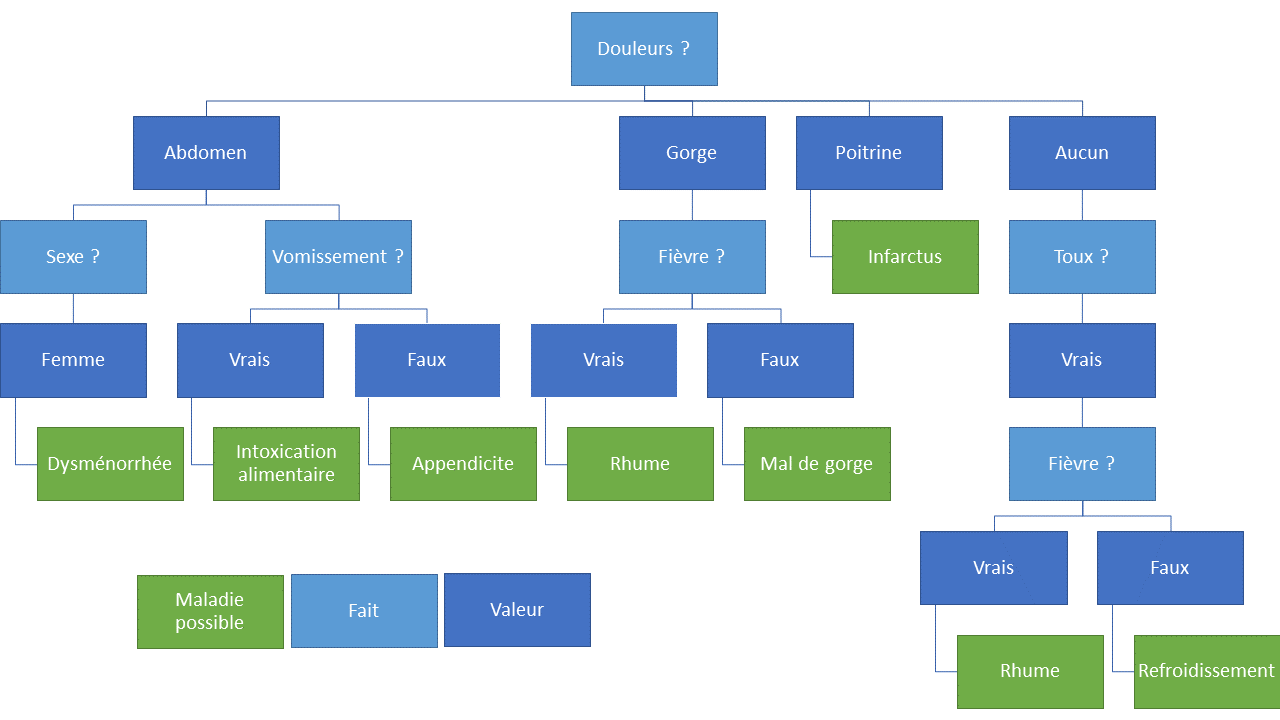
\includegraphics[width=15cm]{arbre.png}
    \caption{\label{arbre} Arbre décisionnel}
\end{figure}

\section{Choix du langage}

Nous avons choisi de partir sur du python car il présente l'avantage d'être fortement typé mais également d'être dynamique ce qui nous permet facilement de gérer les valeurs qui sont de natures différentes.

Pour l'interface, nous nous sommes servis du package pyside2 qui permet d'utiliser, en python, Qt que nous avons déjà vus en C++, et qui en est le package officiel.

\part{Système Expert}

\section{Base de connaissances}

Notre base de connaissances est constitué de la base de faits et la base de règles qui correspondant à des tableaux de faits et de règles.

Elle peut être enrichie à l'aide de fichiers ou bien de l'interface.

\subsection{Fichier}

Le fichier permet de déclarer des faits et des règles (voir en-dessous).
On ne peut avoir qu'un fait ou une règle par ligne mais aussi écrire une ligne de commentaires avec le symbole '\#'.

Pour ce qui est des propositions, on peut aussi ajouter des ou (exprimé ainsi '||') et des parenthèses. Les parenthèses nous ont posé un problème. En effet, nous avons été obligés de convertir nos expressions in-fixe en post-fixe pour pouvoir les calculer.  

\inputminted{sql}{../maladies.txt}

\subsection{Interface}

Selon l'interface, plusieurs méthodes sont disponibles seulement, la plus simple est de taper une ligne comme vous pouvez le faire dans le fichier et de valider.

\section{Moteur d'inférences}

Nous avons implémenté le chaînage avant avec but ou juste pour sature la base de connaissances et le chaînage arrière.

À la fin de l'exécution, il affiche un résultat et le cheminement selon la configuration (changeable). Il est possible de voir le log en tapent la commande "log" et pour lire toutes les commandes disponibles, il suffit de taper "aide".

\section{Interface utilisateur}

Nous avons développé deux interfaces, une en ligne de commandes et une graphique. 

\subsection{Ligne de commandes}

\begin{figure}[H]
    \centering
    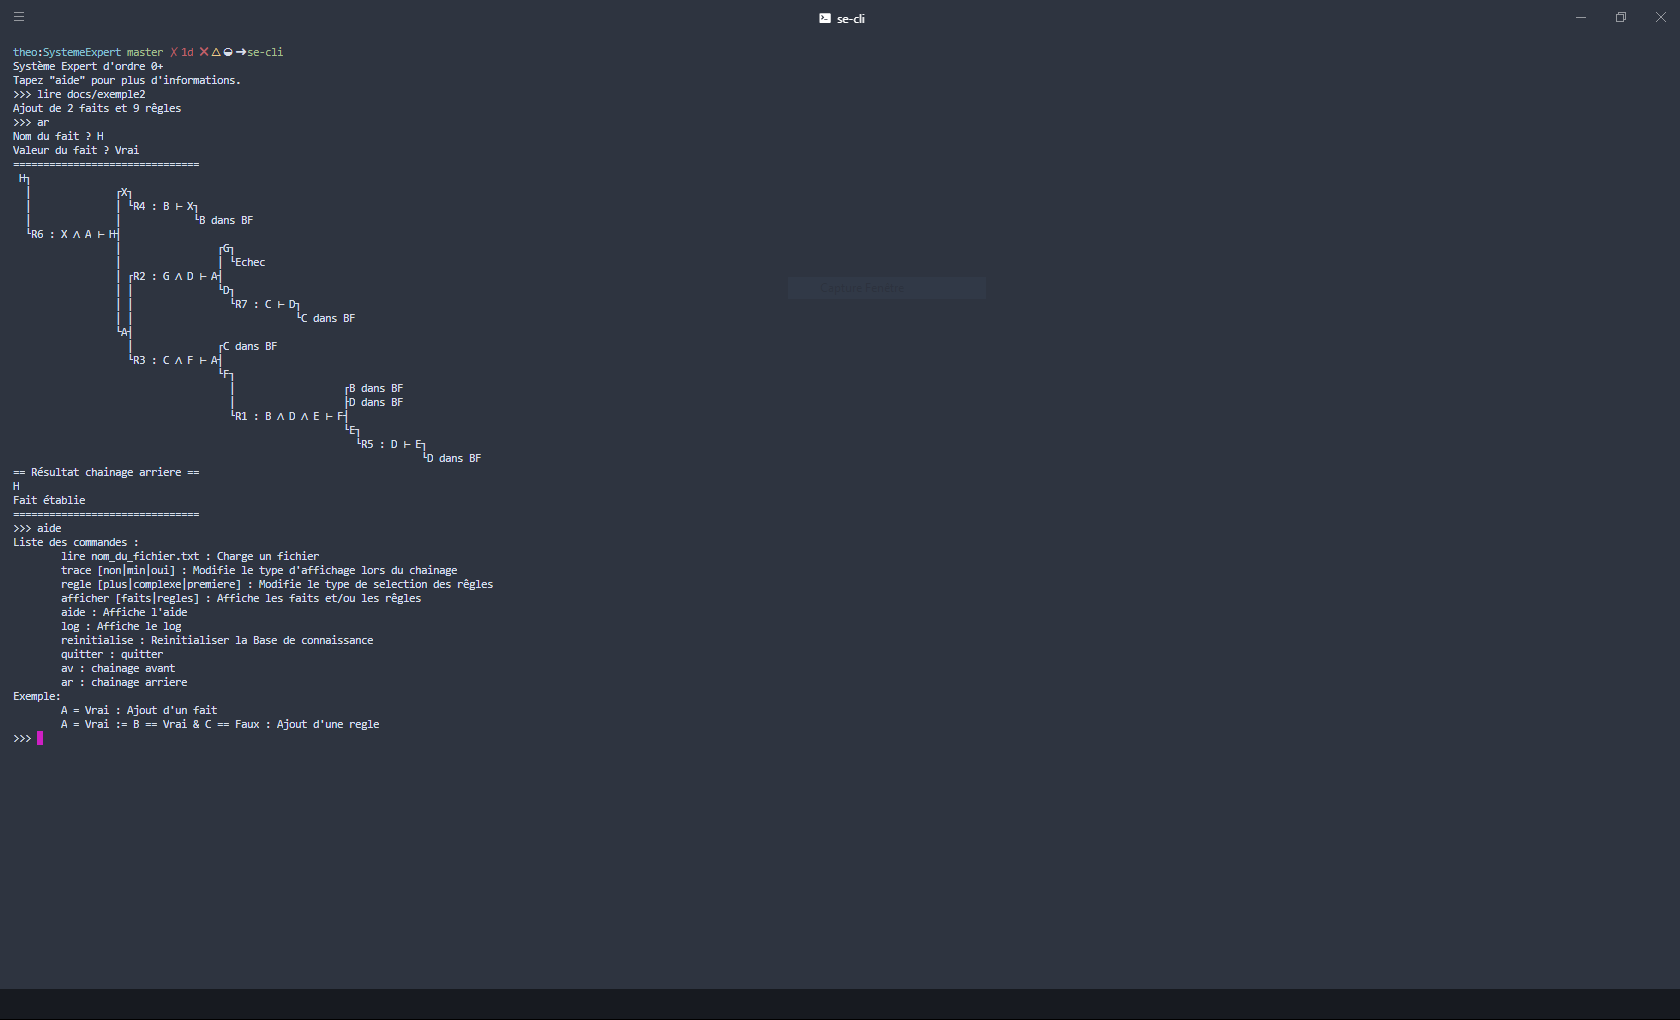
\includegraphics[width=12cm]{cli.png}
    \caption{\label{cli} SE-CLI}
\end{figure}

L'interface une ligne de commandes s'inspire de l'interpréteur de python. Elle permet de faire tout ce que proposes l'interface graphique. Comme l'interpréteur de python, il lit chaque ligne comme si c'était une ligne d'un fichier.

\subsection{Graphique}

\begin{figure}[H]
    \centering
    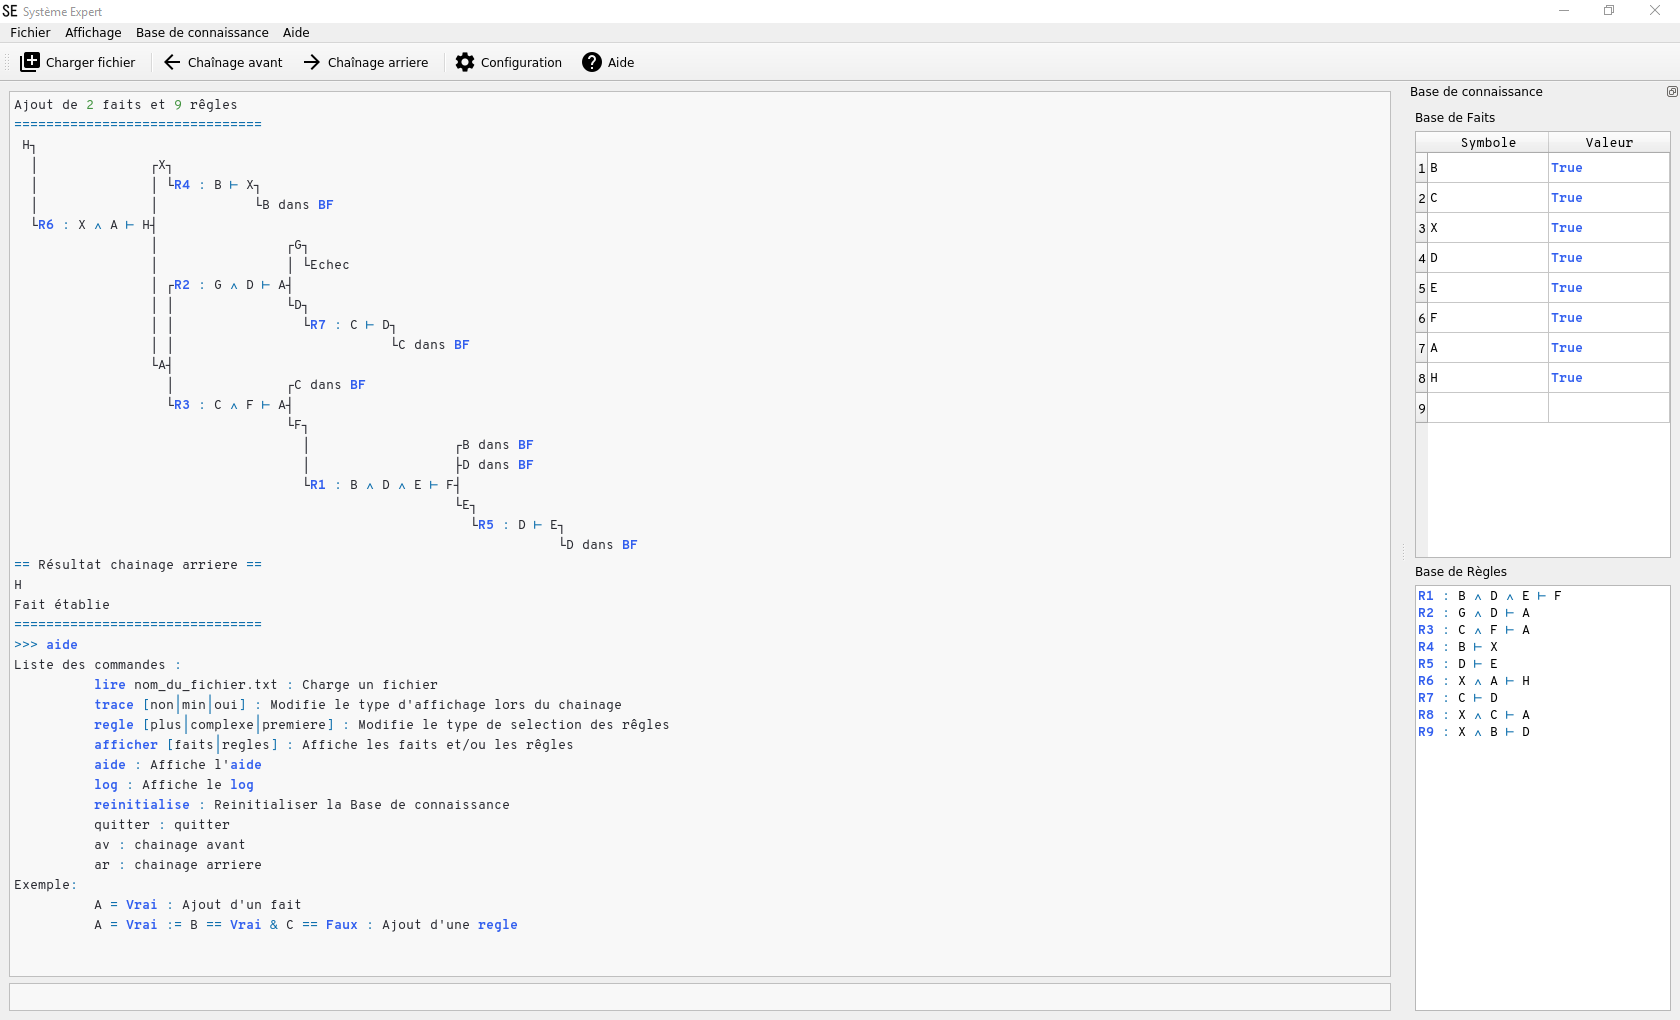
\includegraphics[width=12cm]{gui.png}
    \caption{\label{gui} SE-GUI}
\end{figure}

L'interface permet de simplifier l'utilisation pour un utilisateur qui n'est pas habitué à manipuler un terminal.

La plupart des commandes peuvent être exécutées à l'aide de boutons. Bien sûr, il est toujours possible de taper les commandes comme sur la version en ligne de commandes.

\paragraph{Composition de l'interface}

\begin{description}
    \item[Terminal] Il est constitué d'un affichage et d'une ligne de saisie. Il s'utilise exactement comme la version en ligne de commandes.
    \item[Dock] Il permet d'afficher la base de connaissances et de ajouter/modifier un fait.
    \item[Barre d'outils] Elle donne accès aux commandes importantes.
\end{description}

\part{Conclusion}

\section{Améliorations possibles}

Voici une liste des améliorations possibles:

\begin{itemize}
    \item Ajouter des coefficients de certitude. Pour représenter des événements incertains.
    \item Représenter les faits sous la forme de n-uplet pour faciliter les regroupements des faits. Exemple : AgeBob = 25 devient (Bob,age,25) ou ParentsBob = "Léo Léa" devient (Bob,parents,Léo,Léa).
    \item Transformer le moteur 0+ en 1.
\end{itemize}

\section{Code source du projet}

Toutes les sources du projet et ce document sont disponibles sur \url{https://github.com/theodeze/SystemeExpert}

De plus le projet est disponible sur pypi à l'adresse \url{https://pypi.org/project/sysexpert}. Il suffit de taper cette commande pour télécharger le projet.

\begin{minted}{bash}
    pip install sysexpert
    se-cli # Interface en ligne de commande
    se-gui # Interface graphique
\end{minted}

\end{document}